\subsubsection*{Control Chemotherapy for HIV} 
	Now we discuss a optimal control mode to describe the effect of chemotherapy
in the interaction between the HIV virus and $CD4^+T$ cells 
\cite{butler1997optimal}.


The optimal control problem reads:
\begin{equation} \label{eqn:hiv_infect}
	\begin{aligned}
		\max_{u} & \int_{0}^{t_{final}}
			A  T(t) - (1-u(t)) ^ 2 dt
		\\
		\text{s.t. }
		\\
			T'(t) &=
				\frac{s}{1 + V(t)}
				- m_1 T(t) 
				+ r T(t)
				\left[
					1 - \frac{T(t)+ T_{I}(t)}{T_{max}}
				\right] 
				- u(t) k V(t) T(t),
			\\
			T_{I}(t) &=
				u(t) k V(t) T(t) - m_2 T_{I}(t),
			\\
			V'(t) &= N m_2 T_{I}(t) - m_3 V(t),
			\\
	\end{aligned}
\end{equation}


\begin{table}
	\centering
	\begin{tabular}{rll}
		\toprule
			&\textbf{Description} & \textbf{Value}
            \\
        \midrule
		$\mu_1$ 
        	& Death rate of uninfected $CDT^+T$ cells
        	& \SI{0.02}{d^{-1}} 
            \\
		$\mu_2$ 
       		& Death rate of infected $CDT^+T$ cells
		    & \SI{0.2}{d^{-1}}
			\\
		$\mu_3$ 
      		& Death rate of free virus
		    & \SI{4.4}{d^{-1}}
            \\
        $k$ 
        	& rate $CD4^+T$ cells become infected by free virus
        	& \SI{0.000024}{\milli\meter^3 d^{-1}}
 			\\
		$r$ 
			& rate of growth for the $CD4^+T$ cell population
			& \SI{0.03}{d^{-1}}
     	    \\
     	$N$ 
     		& Number of free virus produced by infected cells
     		& \num{300}
            \\
     	$T_{\max{}}$ 
     		& Maximum $CD4^+T$ cell population level
     		& \SI{1500}{\milli \meter ^ {-3}}
     		\\
     	$s$ 
     		& Source term for uninfected $CD4^{+}T$ cells
     		& \SI{10}{d^{-1}\milli \meter ^{-3}}
		\\
		\\
	    &&
	    \textbf{Initial conditions}
	    \\
	    \cmidrule{3-3}
	    && $T(0) = \num{806.4}$
	    \\
	    && $T_{I}(0)=\num{0.04}$
	    \\
	    && $V(0)= \num{1.5}$
	    \\
		\bottomrule
    \end{tabular}
	\caption{
		Description and simulation parameters for the optimal control model
		\eqref{eqn:hiv_infect}.
	}
	\label{tbl:hiv_infect}
\end{table}






\begin{figure}[tbh]
\centering
	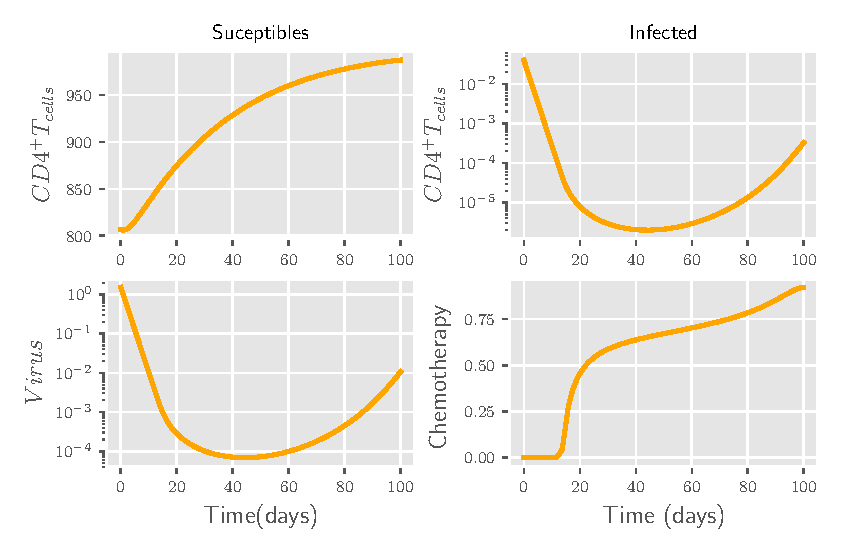
\includegraphics[width=0.7\linewidth]{Figures/hiv_chemotherapy_fig_01}
	\caption{Add description and stress the schedule of treatment}
	\label{fig:hivchemotherapyfig01}
\end{figure}
